% 2010 年湖北卷理科第 13 题：圆柱形容器内三个相同的小球，水面恰好淹没最上面的球。
% 来源 PDF：普通高考/2010/2010湖北理.pdf，SHA-256 2cfb3d100d55f89c58fe4475caf29f039496afbd0f16d7a7d07857eed5759f55。
% 原页：第 1 页（A3 三栏）第 2 栏下部，书页码 597。
% 重绘依据：按 600 dpi 原页，容器画成开口圆筒（两条竖壁 + 底板，无椭圆口），
%   三球直径等于圆筒内径且上下相切，水面横线经过最上面一球的最高点；
%   竖壁略高出水面。球的半径为 r 时坐标取球心 (0,r)、(0,3r)、(0,5r)，水面 y=6r。
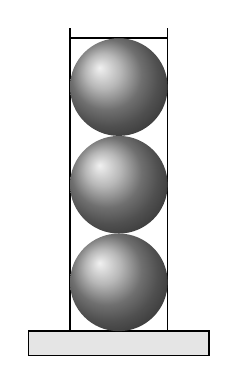
\begin{tikzpicture}[scale=0.62, semithick, every node/.style={inner sep=1.6pt, font=\small}]
  % 底板
  \draw[fill=gray!20] (-1.85,-0.5) rectangle (1.85,0);
  % 圆筒竖壁
  \draw (-1,0) -- (-1,6.2);
  \draw (1,0) -- (1,6.2);
  % 水面
  \draw (-1,6) -- (1,6);
  % 三个球
  \shade[ball color=gray!75] (0,1) circle (1);
  \shade[ball color=gray!75] (0,3) circle (1);
  \shade[ball color=gray!75] (0,5) circle (1);
\end{tikzpicture}
